Wie in der Einführung bekanntgegeben, werden in dieser Arbeit verschieden Methoden zur Evaluierung angewendet. Durch diese mehrfachen Vergleiche können unterschiedliche Wetterphänomene nachgewiesen werden:\\
\begin{table}[h!]
	\begin{tabularx}{\textwidth}{|X|X|X|}
		\hline
		\textbf{Methode} & \textbf{nachgewiesenes Phänomen}& \textbf{Einschränkungen}\\
		\hline
		Jahresmittel [Kap. \ref{chap:mean}] & Übereinstimmung der geographischen Regenzonen im Mittel, und damit lokalisieren von Regionen größere Abweichung ohne auf Starkregenereignisse zu sehr Bezug zu nehmen & Starkregenereignisse können nicht evaluiert werden.\\
		\hline
		Alljährliche 99. Quantile [Kap. \ref{chap:quantile}] & Übereinstimmung der stärksten modellierten Starkregen und Starkregen-Zonen & Besonderheiten der Jahreszeiten können nicht mitbetrachtet werden. Es kann nicht auf kleine Gebiete eingegangen werden, da durch die lange Zeitspanne die Vergleiche verfälscht würden.\\
		\hline
		99. Quantile der Jahreszeiten [Kap. \ref{chap:quantile_seasons}] & Übereinstimmung der Starkregen-Zonen aufgelöst auf Jahreszeiten. Einzelne Gebiete können genauer betrachtet werden. & Einige Starkregenereignisse können nicht allein mit Temperatur und Niederschlag evaluiert werden. Globaler Zusammenhang von Hoch-und Tiefdruck-Gebieten wird vernachlässigt\\
		\hline
	\end{tabularx}
\caption{Verwendete Evaluierungsmethoden}
\end{table}
\hfill\\
Um die Beobachtungsdaten aus dem APGD\cite{meteoswiss} Datensatz mit den simulierten Daten (EUR-11) vergleichen zu können wurden die Beobachtungsdaten mittels cdo (für weitere Informationen siehe \cite{cdo}) auf dasselbe Raster wie die Simulationsdaten gebracht. Dies geschah über eine Interpolation. Für einen bildliche Darstellung siehe: Abb.\ref{fig:interpolieren}. Zum interpolieren wurde die Funktion ''ramapbil'' von cdo verwendet, die eine bilineare Interpolation des gröberen Datengitters auf das feiner vornahm. Das heißt, dass zunächst eine lineare Interpolation in die eine und dann in die andere Richtung vorgenommen wurde, dabei wurde der Abstand einer feineren Gitterzelle zu den Mittelpunkten der umgebenden gröberen Gitterzelle als Gewicht der Interpolation genommen. So wurde ein feineres über den Abstand gemitteltes Gitter aus dem Gröberem errechnet.\\
Um die Daten des simulierten ALP-3 Datensatzes mit den Beobachtungsdaten (APGD \cite{meteoswiss}) vergleichen zu können wurden die Simulationsdaten auf ein gröberes 5x5km Gitter aggregiert: dies geschah über die Funktion remapcon von cdo. Diese Funktion entspricht einem konservativem remappen (für eine vereinfachte Darstellung siehe Abb.\ref{fig:aggregieren}). Laut Definition \cite{remapcon} ist ein remapping operator $R$ konservativ, wenn die globale Masse einer jeden Zelle über das remappen gleich bleibt: somit wird durch das remappen kein zuzüglicher Massefluss erzeugt sondern es wird darauf geachtet, dass über das gesamte Gitter der agglomerierte Massefluss gleich bleibt. (z.B. ist die Summer der Gitter-Weights für beide, grob- und feines Gitter gleich 42)
\begin{figure}[h]
	\begin{subfigure}{0.49\textwidth}
		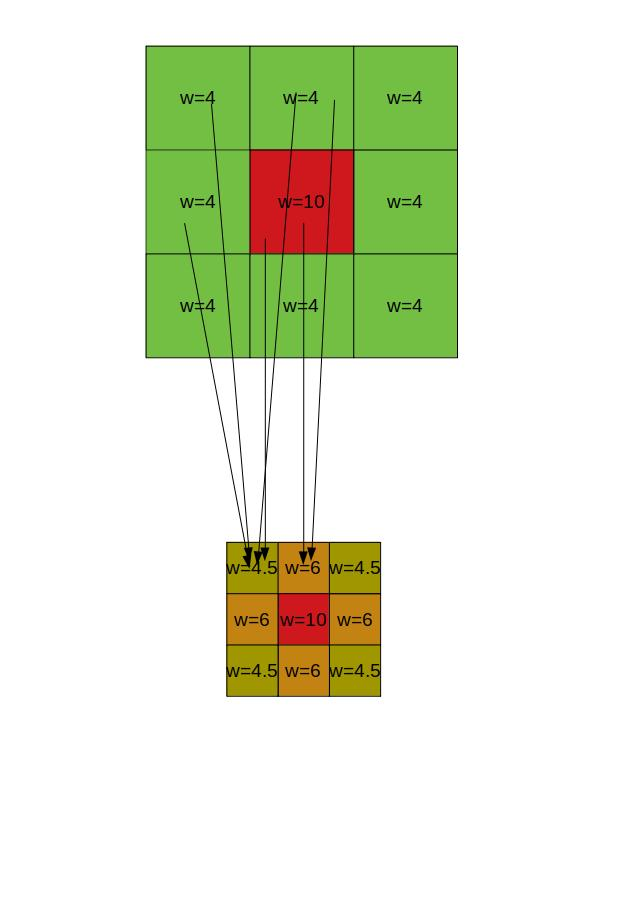
\includegraphics[width=\textwidth]{interpolieren.jpg}
		\caption{Stark vereinfachte Darstellung einer Interpolation}
		\label{fig:interpolieren}
	\end{subfigure}
	\begin{subfigure}{0.49\textwidth}
		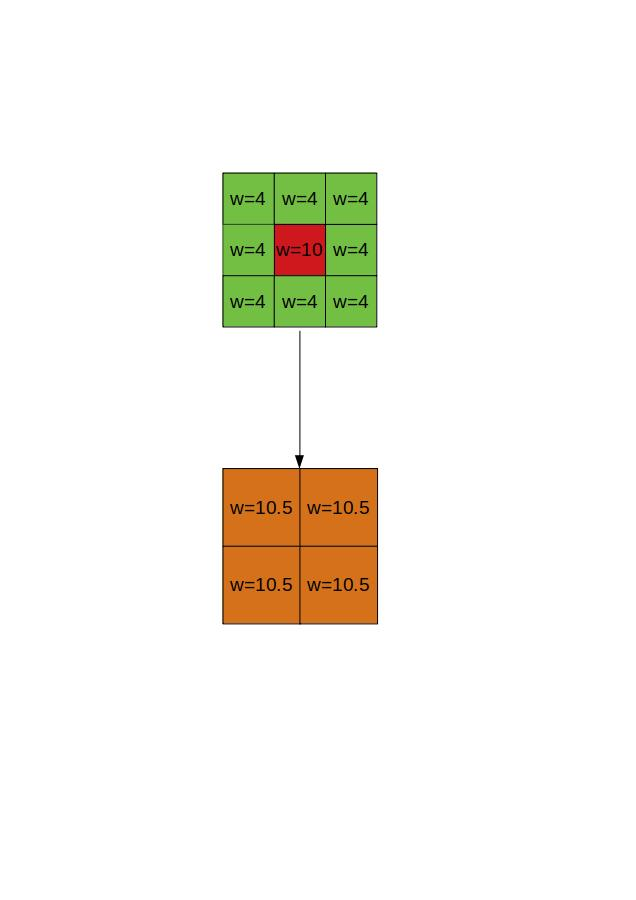
\includegraphics[width=\textwidth]{aggregieren.jpg}
		\caption{Stark vereinfachte Darstellung einer Aggregation (konservatives Remapping)}
		\label{fig:aggregieren}
	\end{subfigure}
	\caption{}
\end{figure}